\documentclass{article}
\usepackage{pgfplots}
\pgfplotsset{compat=1.18}
\usepackage[T1]{fontenc}
\usepackage{sansmathfonts}
\usepackage{caption}

\begin{document}
\begin{center}
  \begin{minipage}[t]{0.30\textwidth}
    \centering
    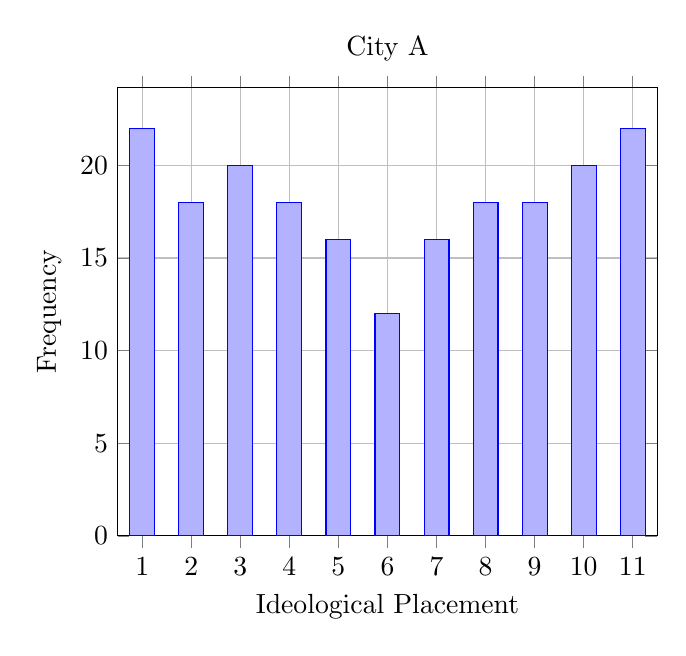
\begin{tikzpicture}
      \begin{axis}[
          ybar,
          bar width=9pt,
          ylabel={Frequency},
          xlabel={Ideological Placement},
          ymin=0,
          xtick=data,
          xticklabels={1,2,3,4,5,6,7,8,9,10,11},
          title={City~A},
          enlarge x limits=0.05,
          grid=major
        ]
        \addplot coordinates {(1,22) (2,18) (3,20) (4,18) (5,16) (6,12) (7,16) (8,18) (9,18) (10,20) (11,22)};
      \end{axis}
    \end{tikzpicture}
  \end{minipage}\hfill
  \begin{minipage}[t]{0.30\textwidth}
    \centering
    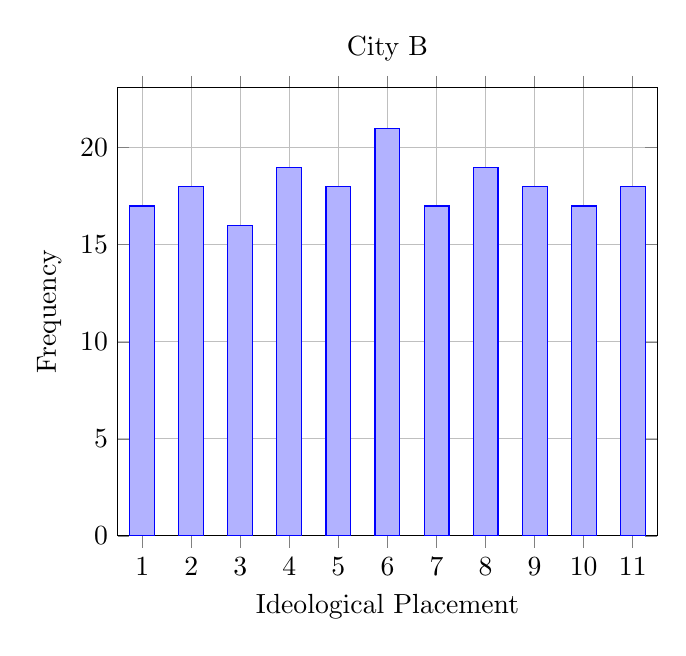
\begin{tikzpicture}
      \begin{axis}[
          ybar,
          bar width=9pt,
          ylabel={Frequency},
          xlabel={Ideological Placement},
          ymin=0,
          xtick=data,
          xticklabels={1,2,3,4,5,6,7,8,9,10,11},
          title={City~B},
          enlarge x limits=0.05,
          grid=major
        ]
        \addplot coordinates {(1,17) (2,18) (3,16) (4,19) (5,18) (6,21) (7,17) (8,19) (9,18) (10,17) (11,18)};
      \end{axis}
    \end{tikzpicture}
  \end{minipage}
\end{center}
\end{document}
